\subsection{Measurement Errors and their Effect on the Parameter Recovery} \label{sec:results_errors}

Measurement uncertainties in proper motions and distance dominate over uncertainties in position on the sky (RA and DEC) and line-of-sight velocity, which can be more accurately determined.

We first investigate the impact of (perfectly known) proper motion uncertainties on the precision of the potential parameter recovery. Figure \ref{fig:isoSphFlexErrConv_SE_vs_error} demonstrates that for data sets with $\delta \mu$ as high as $5~\text{mas yr}^{-1}$ the precision degrades by  a factor of no more than $\sim2$ as compared to a data set without measurement uncertainties. The precision gets monotonically better for smaller $\delta \mu$, being larger only by a factor of $\sim 1.15$ at $\delta \mu=1~\text{mas yr}^{-1}$. With relative standard errors on the recovered parameters of only a few percent at most for 10,000 stars, this means we still get quite precise constraints on the potential, as long as we know the proper motion uncertainties perfectly.

We also note that in this case the relative and absolute difference in recovered precision between the precise and the measurement uncertainty-affected data set does not seem to depend strongly on the kinematic temperature of the stellar population.

Secondly, we investigate the impact of additional measurement uncertainties in distance (modulus). In absence of distance uncertainties the uncertainty-convolved likelihood given in Equation \ref{eq:errorconv} is unbiased.  When including distance (modulus) uncertainties, Equation \ref{eq:errorconv} is just an approximation for the true likelihood. The systematic bias thus introduced in the parameter recovery gets larger with the size of the error, as demonstrated in Figure \ref{fig:isoSphFlexErrConv_bias_vs_SE}.  We find however that in case of $\delta(m-M) \lesssim 0.2 \text{ mag}$ (if also $\delta \mu \lesssim 2 \text{ mas yr}^{-1}$ and a maximum distance of $r_\text{max} = 3 \text{ kpc}$, see Test \ref{test:isoSphFlexErrConv_bias_vs_SE} in Table \ref{tbl:tests}) the potential parameters can still be recovered within 2 sigma \Wilma{[TO DO: Make sure this is what I claim in abstract and discussion.]}. This corresponds to a relative distance error of $\sim10\%$. The overall precision of the potential recovery is also not degraded much by introducing distance uncertainties of less than $10\%$.

We therefore found that in case we perfectly knew the measurement errors (and the distance uncertainty is negligible), the convolution of the model probability with the measurement uncertainties gives precise and accurate constraints on the model parameters - even if the measurement uncertainty itself is quite large.

Lastly, Figure \ref{fig:isoSphFlexErrSyst} now investigates the effect of a systematic \emph{underestimation} of the true proper motion uncertainties $\delta \mu$ by 10\% and 50\%. We find that this causes a bias in the parameter recovery that grows seemingly linear with $\delta \mu$. For an underestimation of only $10\%$ however, the bias is still $\lesssim 2$ sigma for 10,000 stars \Wilma{[TO DO: Check]} - even for $\delta \mu \sim 3~\text{mas yr}^{-1}$.

The size of the bias also depends on the kinematic temperature of the stellar population and the model parameter considered (see Figure \ref{fig:isoSphFlexErrSyst}). The qDF parameters are for example better recovered by hotter populations. This is, because the \emph{relative} difference between the true $\sigma_i(R)$ (with $i \in \{R,z\}$) and measured $\sigma_i(R)$ (which comes from the deconvolution with an underestimated velocity uncertainty) is smaller for hotter populations. 

%=============================================================

\begin{figure}[!htbp]
\centering
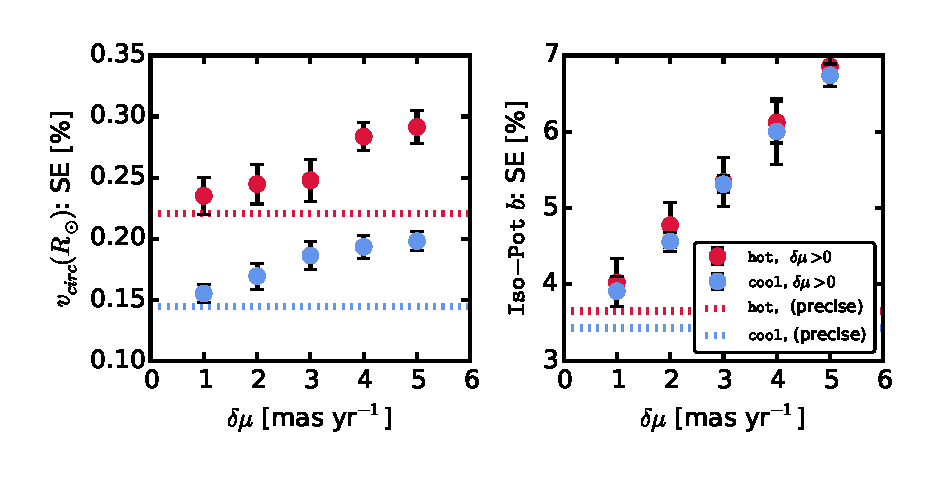
\includegraphics[width=\columnwidth]{figs/isoSphFlexErrConv_SE_vs_error.eps}
\caption{Effect of proper motion uncertainties $\delta \mu$ on precision of potential parameter recovery for two stellar populations of different kinematic temperature (see Test \ref{test:isoSphFlexErrConv_SE_vs_error} in Table \ref{tbl:tests} for all model parameters). The relative standard error (SE) derived from the marginalized \pdf{} for each model parameter was determined for precise data sets without measurement uncertainties (solid lines, with dotted lines indicating the error) and for data sets affected by different proper motion uncertainties $\delta \mu$ and $\delta v_\text{los}=2~\text{km s}^{-1}$ (data points with errors), but no uncertainties in position. The errors come from taking the mean over the results from several data sets.}
\label{fig:isoSphFlexErrConv_SE_vs_error}
\end{figure}


%=============================================================

\begin{figure}[!htbp]
\centering
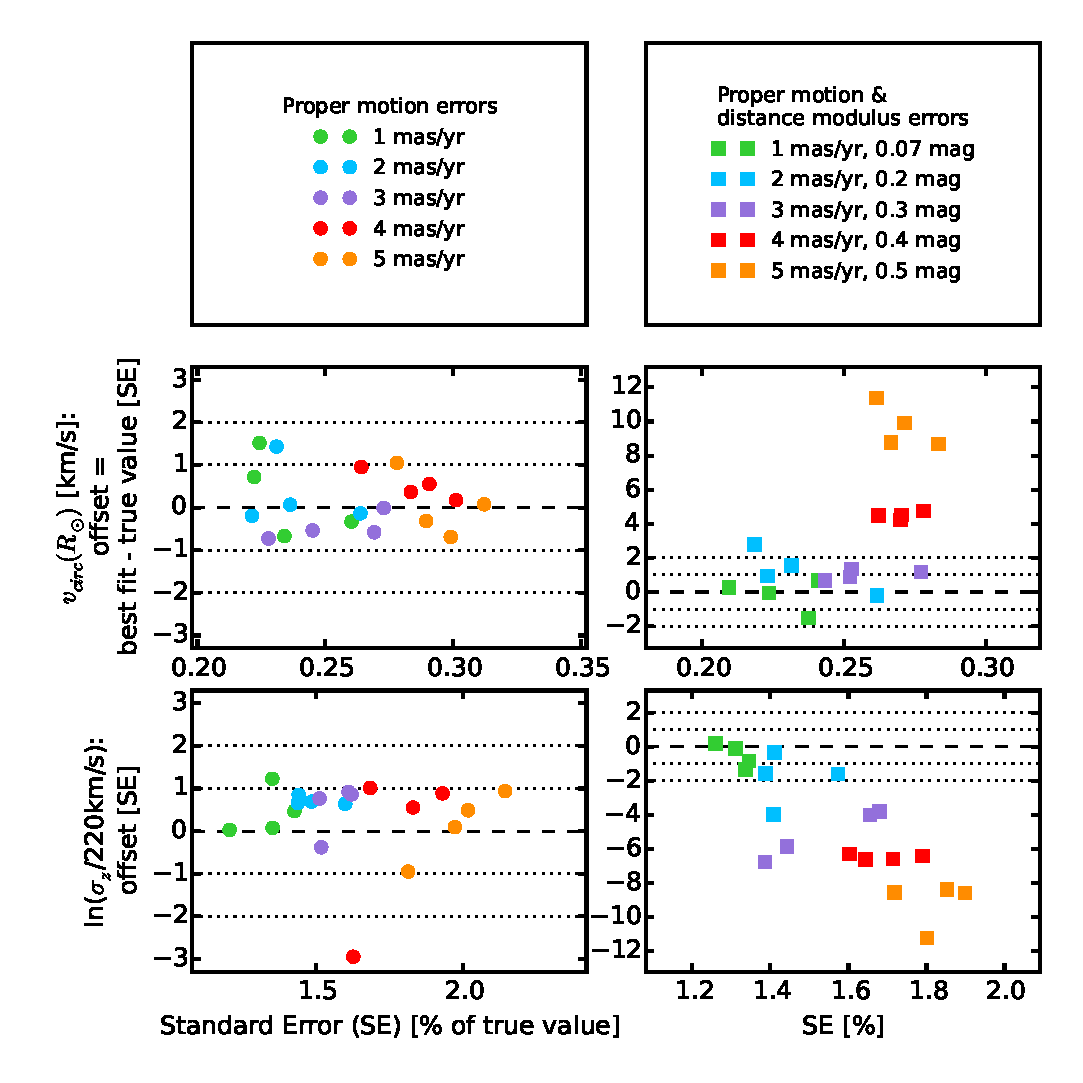
\includegraphics[width=\columnwidth]{figs/isoSphFlexErrConv_bias_vs_SE.eps}
\caption{Potential parameter recovery using the approximation for the model probability convolved with measurement uncertainties in Equation \ref{eq:errorconv}. We show  \pdf{} offset and relative width (i.e., standard error SE) for the potential parameters derived from mock data sets, which were created according to Test \ref{test:isoSphFlexErrConv_bias_vs_SE} in Table \ref{tbl:tests}). The data sets in the left panels have only uncertainties in line-of-sight velocity and proper motions, while the data sets in the right panels also have distance (modulus) uncertainties, as indicated in the legends in the first row. For data sets with proper motion error errors $\delta(m-M) \leq 3 \ \text{mas yr}^{-1}$ Equation \ref{eq:errorconv} was evaluated with $N_\text{error}=800$, for $\delta(m-M) > 3 \ \text{mas yr}^{-1}$ we used $N_\text{error}=1200$. In absence of distance uncertainties Equation \ref{eq:errorconv} gives unbiased results. For $\delta(m-M) \geq 3 \text{mas yr}^{-1}$ (which corresponds in this test to $\delta v_\text{max} \lesssim 43 \ \text{km s}^{-1}$, see Equation \ref{eq:vmax}) however biases of several sigma are introduced as Equation \ref{eq:errorconv} is only an approximation for the true likelihood in this case.}
\label{fig:isoSphFlexErrConv_bias_vs_SE}
\end{figure}




%=============================================================

\begin{figure}[!htbp]
\centering
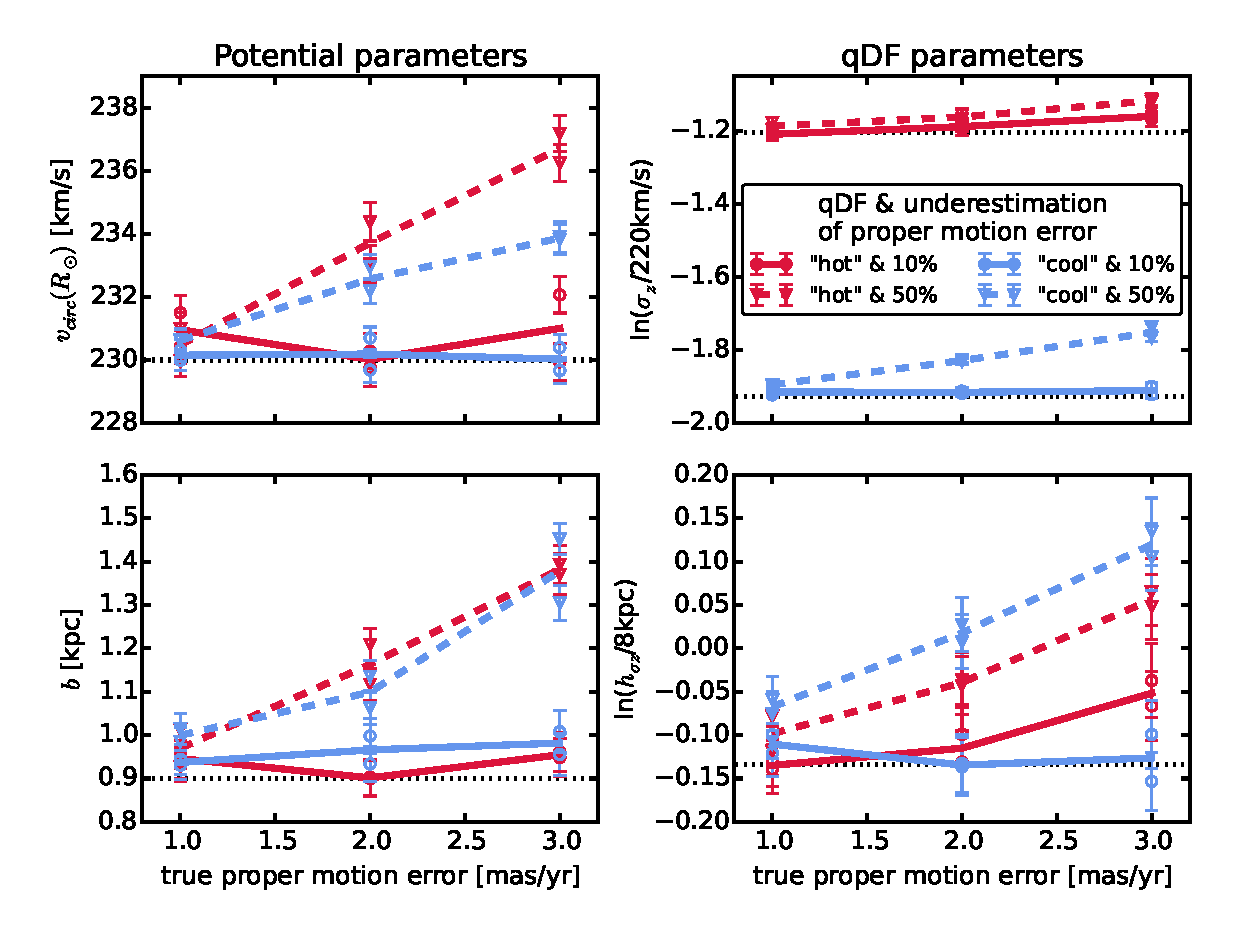
\includegraphics[width=\columnwidth]{figs/isoSphFlexErrSyst_offset_vs_error.eps}
\caption{Effect of a systematic underestimation of proper motion errors in the recovery of the model parameters. The true model parameters used to create the mock data are summarized as Test \ref{test:isoSphFlexErrSyst} in Table \ref{tbl:tests}, four of them are given on the $y$-axes and the true values are indicated as black dashed lines. The velocities of the mock data were perturbed according to Gaussian errors in the RA and DEC proper motions as indicated on the $x$-axis. The circles and triangles are the best fit parameters of several mock data sets assuming the proper motion uncertainty, with which the model probability was convolved, was underestimated in the analysis by 10\% or 50\%, respectively. The error bars correspond to 1 sigma confidence. The lines connect the mean of each two data realisations and are just to guide the eye. \Wilma{[TO DO: rename $h_{\sigma z}$ to $h_{\sigma,z}$, $\sigma_z$ to $\sigma_{z,0}$] [TO DO: Potential and/or population names in typewriter font] [TO DO: Iso-Pot in Title] [TO DO: Delta mu on x-axis] [TO DO: legend with true values]}}
\label{fig:isoSphFlexErrSyst}
\end{figure}

%=============================================================

\Wilma{[TO DO: Comment from Jo: Always use 'uncertainty' when describing how ou deal with the errors. 'Error' means the actual error (difference between observed and true).]}
